
\documentclass[12pt,letterpaper]{report}
\usepackage{natbib}
\usepackage{geometry}
%\usepackage{fancyheadings} fancyheadings is obsolete: replaced by fancyhdr. JL
\usepackage{fancyhdr}
\usepackage{afterpage}
\usepackage{graphicx}
\usepackage{amsmath,amssymb,amsbsy, amsthm}
\usepackage{tikz}
\usepackage{dcolumn,array}
\usepackage{tocloft}
\usepackage{asudis}
\usepackage{float}
\usepackage{algorithm, algpseudocode}
\usepackage{caption}
\usepackage[edges]{forest}
\usepackage{subcaption}
\theoremstyle{plain}
\newtheorem{theorem}{Theorem}
\newtheorem{corollary}[theorem]{Corollary}
\newtheorem{lemma}[theorem]{Lemma}
\newtheorem{proposition}[theorem]{Proposition}
\theoremstyle{definition}
\newtheorem{definition}[theorem]{Definition}
\newtheorem{example}[theorem]{Example}
\newtheorem{conjecture}[theorem]{Conjecture}

\newcommand{\x}{{\mathbf{{x}}}} 
\newcommand{\dotx}{{\mathbf{\dot{x}}}} 
\newcommand{\ddotx}{{\mathbf{\Ddot{x}}}} 
\renewcommand{\u}{\mathbf{\hat{u}}}
\renewcommand{\H}{{\mathbf{H}}}
\newcommand{\Hb}{{\mathbf{H_B}}}
\newcommand{\F}{{\mathbf{F}}}
\newcommand{\Fn}{{\mathbf{F_n}}}
\newcommand{\Fc}{{\mathbf{F_n}}}
\renewcommand{\d}{{\mathbf{d}}}
\newcommand{\db}{{\mathbf{d_B}}}
\newcommand{\ZERO}{{\mathbf{0}}}
\newcommand{\EYE}{{\mathbf{I}}}
\newcommand{\Lie}{\pounds}
\newcommand{\IHat}{\hat{I}}
\newcommand{\ITilde}{\Tilde{I}}
\newcommand{\B}{\mathbf{B}}
\newcommand{\BL}{^\mathbf{B-1}_\mathbf{B-1}}
\newcommand{\BB}{^\mathbf{B}_\mathbf{B}}
\newcommand{\com}{\mathbf{c}}
\newcommand{\M}{\mathbf{M}}
\newcommand{\dB}{\dot{\B}}
\newcommand{\transpose}{^\intercal}
\newcommand{\f}{\mathbf{f}}
\newcommand{\g}{\mathbf{g}}
\renewcommand{\S}[1]{\mathring{S}\left(#1\right)}
\newcommand{\Sn}[1]{\mathring{S_3}\left(#1\right)}
\newcommand{\X}{\mathbf{X}}
\renewcommand{\r}{\mathbf{r}}
\newcommand{\dotr}{\dot{\r}}
\newcommand{\dotX}{\dot{\X}}
\newcommand{\tensor}[1]{\mathbf{\Bar{#1}}}
\newcommand{\partialX}[1]{\frac{\partial#1}{\partial\X}}
\newcommand{\partialx}[1]{\frac{\partial#1}{\partial\x}}
\newcommand{\partialxdot}[1]{\frac{\partial#1}{\partial\dotx}}
\newcommand{\T}{\mathbf{T}}
\renewcommand{\P}{\mathbf{P}}



\DeclareMathOperator*{\argmax}{argmax}
\DeclareMathOperator*{\argmin}{argmin}
%\DeclareMathOperator{\Hessian}{\mathbf{H}}
%\DeclareMathOperator{\J}{\mathbf{J}}
\newcommand{\Hessian}{\mathbf{H}}
\newcommand{\J}{\mathbf{J}}
\newcommand{\dotJ}{\dot{\J}}
\renewcommand{\algorithmicrequire}{\textbf{Input:}}
\renewcommand{\algorithmicensure}{\textbf{Output:}}

\begin{document}

%-----------------------front matter
\pagenumbering{roman}
\title{On the Numerical Computation of Second Order Control Barrier Functions}
\author{Daniel Pietz}
\degreeName{Master of Science in Engineering}
\defensemonth{November}
\gradmonth{December}
\gradyear{2022}
\chair{Dr. Georgios Fainekos, Co-Chair \\ Dr. Sarma Vrudhula, Co-Chair \\ Dr. Theodore Pavlic\\ Dr. Giulia Pedrielli}		
\maketitle
\doublespace
\begin{abstract}Sample Abstract\end{abstract}
\acknowledgementpage{}
%\include{ack}
\tableofcontents
% This puts the word "Page" right justified above everything else.
\addtocontents{toc}{~\hfill Page\par}
% Asking LaTeX for a new page here guarantees that the LOF is on a separate page
% after the TOC ends.
\newpage
% Making the LOT and LOF "parts" rather than chapters gets them indented at
% level -1 according to the chart: top of page 4 of the document at
% ftp://tug.ctan.org/pub/tex-archive/macros/latex/contrib/tocloft/tocloft.pdf

% This gets the headers for the LOT right on the first page.  Subsequent pages
% are handled by the fancyhdr code in the asudis.sty file.
\addcontentsline{toc}{part}{LIST OF TABLES}
\listoftables
\addtocontents{lot}{Table~\hfill Page \par}
\newpage
\addcontentsline{toc}{part}{LIST OF FIGURES}
\listoffigures
\addtocontents{lof}{Figure~\hfill Page \par}
\newpage
\addcontentsline{toc}{part}{LIST OF SYMBOLS}
\clearpage
\symbolspage{}
\addcontentsline{toc}{part}{PREFACE}
\clearpage
\addtocontents{toc}{CHAPTER \par}					
\prefacepage{\\Enter content here.}

% This gets the headers for the LOF right on the first page.  Subsequent pages
% are handled by the fancyhdr code in the asudis.sty file.
%-----------------------body
\doublespace
\pagenumbering{arabic}
\chapter{INTRODUCTION}

\section{Motivation}
 
Between 2010 and 2020, the number of robotic systems in industrial applications nearly tripled, from 1.06 million units to over 3 million \Cite{richter_2021}. This growth is not limited to industrial applications, with the common individual beginning to interact with robotics systems daily. The year 2017 saw the first commercial launch of Starship Technologies, a food delivery robot typically deployed at college campuses \Cite{Kottasova}. More high-stakes, complex, applications are beginning to be automated as well. These include cleaning up from nuclear meltdowns \Cite{stahl_2021}, heart surgeries \Cite{mayo_2022}, and self-driving cars \Cite{thrun_2010}. Such an increase in quantity and complexity brings two risks: an increase in the number of failures, and an increase in the consequences of failures. Thus, there is a growing necessity to implement control systems capable of guaranteeing the safety of a system. Control Barrier Functions (CBFs) were developed to address this need \Cite{Ames1}, however, their computational complexity makes their implementation infeasible for many real-time applications. In order to fully utilize CBFs, a more efficient implementation is needed.\newline

\section{Contribution of the Thesis}

 In this thesis, I present a novel algorithm, the \algname{} algorithm for implementing second-order control barrier functions on any rigid open kinematic chain.

 \section{Thesis Structure}
 
 Chapter \ref{chap:Background} introduces the notation and background knowledge necessary for communicating the \algname{} algorithm. Chapter \ref{chap:Kinematics} outlines the dynamics algorithm used for numerically evaluating the equations of motion of an open kinematic chain \Cite{isenberg_2020}.  Chapter \ref{chap:differential_kinematics} contains the derivation of the gradient dynamics for computing terms necessary for second-order control barrier functions. Chapter \ref{chap:implementation} shows how the dynamics and \algname{} algorithms can be used to implement a second-order CBF on any rigid open kinematic chain. Chapter \ref{chap:examples} contains simulations to compare this implementation against symbolic execution for different types of systems. Finally, Chapter  \ref{chap:conclusions} discusses the author's conclusions and future work on this topic.


%{HOOK LINE, Something about Industry 4.0 and rapidly growing automation}. With this growing industry, comes an increasing level of interaction with autonomous agents {cite some hospital thing}, as well as agents operating without any human guidance outright {Cite spot patrol.}. Because of this, the problem of ensuring such systems achieve their goals in a safe manner is becoming evermore important. To address this, we often categorize our system requirements into two categories, safety and liveliness. As put by Ames, a safe system is one where ``bad'' things do not happen, and a lively system is one where ``good'' things eventually happen (\cite{Ames1}). Safety requirements of often encoded by defining a ``safe set'' representing all states of the system in which bad things do not occur. Similarly, liveliness requirements are defined as a ``goal set'' , representing states we wish our system to eventually achieve. With definitions for these sets defined, the next challenge is designing a control system guaranteeing that trajectories within the safe-set can never leave, whilst also eventually entering the goal set. To solve this, Control Barrier Functions (CBF) and Control Lyaponov Functions (CLF) were developed.

\chapter{BACKGROUND} \label{chap:Background}
\section{Notation}

\begin{definition} \label{tensor_indexing}
\noindent For a tensor of rank 3 $\tensor{A}$, let $\tensor{A}_{i,j,k}$ denote the element at the $i$-th page, $j$-th row, and $k$-th column.

\begin{figure}[H]
    \centering
    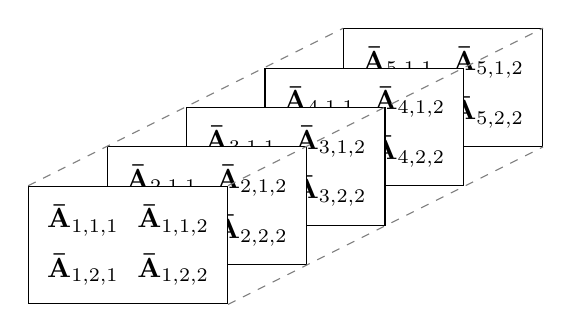
\begin{tikzpicture}
\def\xs{1} %shift in x direction
\def\ys{0.5} %shift in y direction
\def\nm{5} % number of 2d matrices in the 3d matrix
\foreach \x in {5, 4, 3, 2, 1}
{

\matrix [draw, % for the rectangle border
         fill=white, % so that it is not transparent
         ampersand replacement=\&] %see explanation
(mm\x)%give the matrix a name
at(\x * \xs, \x * \ys) %shift the matrix
{

    \node {$\tensor{A}_{\x,1,1}$}; \& \node {{$\tensor{A}_{\x,1,2}$}} ; \\
    \node {{$\tensor{A}_{\x,2,1}$}}; \& \node {{$\tensor{A}_{\x,2,2}$}};\\
};
}
\draw [dashed,gray](mm1.north west) -- (mm\nm.north west);
\draw [dashed,gray](mm1.north east) -- (mm\nm.north east);
\draw [dashed,gray](mm1.south east) -- (mm\nm.south east);
\end{tikzpicture}
\end{figure}
\end{definition}

\begin{definition} \label{matrix_derivative}
Let $\mathbf{A} \in \mathbb{R}^{m \times n}$ and $\mathbf{\x} \in \mathbb{R}^{p \times 1}$. $\tensor{B} = \frac{\partial}{\partial \x}\mathbf{A} \in \mathbb{R}^{p \times m \times n }$ such that
\begin{align*}
    \tensor{B}_{i, j, k} = \frac{\partial}{\partial \x_i}\mathbf{A}_{j, k}
\end{align*}
\end{definition}

\begin{definition}
Let $\S{\mathbf{v}} : \mathbb{R}^{3} \rightarrow \mathbb{R}^{3 \times n}$  denote the skew symmetric cross product matrix of $\mathbf{v}$ \textbf{s.t}
\begin{align*}
    \S{\mathbf{v}} = \begin{bmatrix}
    0 & -\mathbf{v}_2 & \mathbf{v}_1 \\
    \mathbf{v}_2 & 0 & -\mathbf{v}_0 \\
    -\mathbf{v}_1 & \mathbf{v}_0 & 0
    \end{bmatrix}
\end{align*}
\end{definition}


\begin{definition}
Let $\Sn{\mathbf{B}} : \mathbb{R}^{3 \times n} \rightarrow \mathbb{R}^{n \times 3 \times n}$  \textbf{s.t}  if $\bar{\mathbf{A}} = \Sn{\mathbf{B}}$, then $\bar{\mathbf{A}}_i = \S{\mathbf{B}_{i}}$ where $\mathbf{B}_{i}$ denotes the $i$-th column of $\mathbf{B}$.
\end{definition}

\begin{definition}Let $^A_B\r_C$ denote the position of frame $C$ with respect to frame $B$, measured in frame $A$.
\begin{figure}[H]
    \centering
    \includegraphics[width=0.5\textwidth]{Figures/Intro/FramesNC.png}
    \caption{Position Notation}
    \label{fig:position_notation}
\end{figure}
\end{definition}

\begin{definition}Let $^A\T_B$ denote the rotation matrix of frame $B$ frame A, with columns equating the basis vectors of $B$ measured in $A$.
\end{definition}

\begin{definition}Let $^A_B\omega_C$ denote the angular velocity of frame $C$ with respect to frame $B$, measured in frame $A$.
\end{definition}

\subsubsection{Rigid Bodies}

\begin{definition}
We define a link / rigid body $B$ as an tuple $B = \left (\B, \quad m_\B, \quad \BB\com, \quad \BB\J \right )$ where
\begin{align*}
    \B &:= \text{Frame of reference} \\
    m_\B &:= \text{Mass} \\
    \BB\com &:= \text{Center of Mass measured in/about $\B$} \\
    \BB\J &:= \text{Moment of inertia measured in/about $\B$} \\
\end{align*}
\begin{figure}[H]
    \centering
    \includegraphics[width=0.5\textwidth]{Figures/Intro/BodyFrames.png}
    \caption{Body Notation}
    \label{fig:body_notation}
\end{figure}

\noindent References to a link/body and its frame of reference are used interchangeably throughout this text.
\end{definition}

\subsubsection{Joints}

\begin{definition}
A \textbf{prismatic joint} is a link that actuates on a linear axis.
\end{definition}

\begin{definition}
A \textbf{rotational joint} is a link that actuates on a rotating axis.
\end{definition}

\begin{definition}
An \textbf{open kinematic chain} is a series of connected links containing no closed loops.
\end{definition}


\begin{definition}Let $^A_B\r_C$ denote the position of frame $C$ with respect to frame $B$, measured in frame $A$.
\begin{figure}[H]
    \centering
    \includegraphics[width=0.4\textwidth]{Figures/Intro/OKC.png}
    \includegraphics[width=0.4\textwidth]{Figures/Intro/NOKC.png}
    \caption{Open vs Closed Kinematic Chain}
    \label{fig:okc}
\end{figure}
\end{definition}


\begin{definition}
Let $B-1$ denote the link/body to which a link/body $B$ is attached in an open kinematic chain, off of which measurements are made.
\end{definition}

\section{The Newton Euler Formulation}

The Newton-Euler equations describe the translational and rotational motion of a rigid body through space \Cite{Hahn, asada_slotine_1986, shabana_2010}. Measured with respect to a coordinate frame at the center of mass of a body, 

\begin{align}
    \begin{bmatrix}
    \tau \\ \F
    \end{bmatrix} = 
    \begin{bmatrix}
     {\BB\J} & \ZERO_{3 \times 3} \\
      \ZERO_{3 \times 3} & m \EYE_{3 \times 3}
    \end{bmatrix}
    \begin{bmatrix}
     \mathbf{\dot{\omega}}\\
     \ddotx
    \end{bmatrix}
    + 
    \begin{bmatrix}
     \omega \times {\BB\J}\omega\\
     \ZERO_{3 \times 1} 
    \end{bmatrix}
\end{align}

\noindent Shifting the frame of reference, such that the center of mass is located at $\BB \com$, yields

\begin{align} \label{eqn:NE0}
    \begin{bmatrix}
    \tau \\ \F
    \end{bmatrix} = 
    \begin{bmatrix}
     {\BB\J} & m\S{\BB\com} \\
      -m\S{\BB\com} & m \EYE_{3 \times 3}
    \end{bmatrix}
    \begin{bmatrix}
     \ddotx\\
     \mathbf{\dot{\omega}}
    \end{bmatrix}
    + 
    \begin{bmatrix}
     \S{\omega}{\BB\J}\omega \\
     m \S{\omega}^2{\BB\com}
    \end{bmatrix}
\end{align}

%TODO: CHECK THIS CITATION TO MAKE SURE IT WORKS

\noindent Equation \ref{eqn:NE0} is limited to a single rigid body, however, it provides a starting point to model the motion of more complex systems. Such a model is given by the following equation \Cite{asada_slotine_1986, tedrake}, sometimes referred to as the \textit{Robot Equation} \Cite{isenberg_2020}.
\begin{align} \label{eqn:NE1}
    \H(\x)\ddotx = \F(\x, \dotx) - \d(\x, \dotx)
\end{align}

\noindent $\H$ is a positive definite $n \times n$ matrix, commonly called the System Mass Matrix \Cite{riley_hobson_bence_2006}. $\F$ contains external forces acting on the system, and $\d$ contains the Centrifugal and Coriolis forces, also called fictitious forces. Crucially, equation \ref{eqn:NE1} can be rewritten into a form that is Nonlinear Control Affine. \newline

A nonlinear control-affine system takes the following form
\begin{align} \label{eqn:NLCA}
    \dotx = \f(\x) + \g(\x) \u
\end{align}
\noindent Where $\x \in \mathbb{R}^n$ represents the state space configuration of the system, $\f$ denotes the natural response of the system, and $\g$ maps the control input $\u$ into the generalized coordinate space. $\ref{eqn:NE1}$ can be written into the form of \ref{eqn:NLCA}.
\begin{align*}
    \H \ddotx &= \F  - \d  \\ \nonumber
    \ddotx &= \H^{-1}\left (\F  - \d \right ) 
\end{align*}
\begin{align*} \nonumber
\text{Let  }  \X &= \begin{bmatrix} \x & \dotx \end{bmatrix}\transpose \\
    \dotX &= \begin{bmatrix}
     \dotx &\ddotx
    \end{bmatrix}\transpose 
    =
    \begin{bmatrix}
     \dotx \\ \H ^{-1}\left (\F  - \d \right ) 
    \end{bmatrix} 
    =
    \begin{bmatrix}
     \dotx \\ \H ^{-1}\left (\Fn  + \P\u - \d \right )
    \end{bmatrix} \\
    \text{where } \F &= \Fn  + \P(\x, \dotx)\u 
    \end{align*}
    \begin{align*}
    \dotX =
    \begin{bmatrix}
     \dotx \\ \H ^{-1}\left (\Fn  - \d \right ) + \H ^{-1}\left ( \P\u \right )
    \end{bmatrix} \\ &=
    \begin{bmatrix}
     \dotx \\ \H ^{-1}\left (\Fn  - \d \right )
    \end{bmatrix} + \begin{bmatrix}
     \ZERO_{n \times 1} \\  \H ^{-1} \P\u
    \end{bmatrix} \\
    &=
    \begin{bmatrix}
     \dotx \\ \H ^{-1}\left (\Fn  - \d \right )
    \end{bmatrix} + \begin{bmatrix}
     \ZERO_{n \times n} \\  \H ^{-1}\P
    \end{bmatrix}\u \\
    &= \f(\X) + \g(\X)\u \\
    \text{where } \f(\X) &= \begin{bmatrix}
     \dotx \\ \H ^{-1}\left (\Fn  - \d \right )
    \end{bmatrix} \\ \text{ and } \g(\X) &= \begin{bmatrix}
     \ZERO_{n \times n} \\  \H ^{-1}\P
    \end{bmatrix}
\end{align*}

% TODO: These equations are ugly. Fix the formatting.

\noindent With the system in control affine form allows for the usage of optimization-based controllers, such as Controller Barrier Functions (CBF).

\section{The CBF  - QP}

%TODO: Intro to this section
Control Barrier Functions provide an architecture for safety-aware controllers on nonlinear control affine systems \Cite{Ames1}. Such controllers operate by finding a control input that maintains invariance in the state of a system, $x \in \mathbb{R}^n$ with respect to a safe set, $C \in \mathbb{R}^n$. This safe safe set is represented in the controller through a \textit{barrier function}, $h(x) : \mathbb{R}^n \rightarrow \mathbb{R}$. We define $h(x)$ such that $C$ is a \textit{super-level set} of $h(x)$, yielding
\begin{align}
\begin{split}
    C = \left \{ x \in \mathbb{R}^n | h(x) \geq 0 \right \} 
\end{split}
\begin{split}
\end{split}
\begin{split}
    \partial C = \left \{ x \in \mathbb{R}^n | h(x) = 0 \right \}
\end{split}
\begin{split}
\end{split}
\begin{split}
    \text{Int}(C) = \left \{ x \in \mathbb{R}^n | h(x) > 0 \right \}
\end{split}
\end{align}

\noindent One can then prove safety for a system by showing $\dot{h}(x) \geq 0 \forall x \in \partial C$ \Cite{nagumo_1942}. In the case of nonlinear control affine systems, this is shown by
\begin{align}
    \Lie_f h(x) + \Lie_g h(x)u \geq -\alpha(h(x))
\end{align}
\noindent Where $\alpha(x)$ is a class $\kappa$ function, and $\Lie_p q$ denotes the \textit{Lie Derivative}, $\nabla q \cdot p$. \newline
This requirement can be expressed as a quadratic optimization problem, the goal of which is to find a control input that guarantees invariance of the safe set, shown in the following
\begin{align} \label{eqn:CBF-CLF-QP}
    u(x) = \argmin_{u \in \mathbb{R}^{m}} \quad &\frac{1}{2}(u - u_{ref}))^TH(x)(u - u_{ref})\\
    \textbf{s.t} \quad  &\Lie_f h(x) + \Lie_g h(x)u \geq -\alpha(h(x)) \nonumber
\end{align}

\noindent In this setting, $u_{ref}$ denotes the value of some reference controller on the system. In plain English, the goal of this quadratic program is to find the closest control input to $u_{ref}$ that satisfies the safety constraints of the system. In the case of min-norm controllers, $u_{ref}$ is set to 0. \newline

Note that the controller in Equation \ref{eqn:CBF-CLF-QP} is limited in that it is only applicable to first-order systems. That is systems in which the control input appears in the first derivative. Equation \ref{eqn:NE1} describes a second-order system, prohibiting the use of this controller. To implement a positional controller on these types of systems, High Order CBFs (HOCBF) must be used \Cite{Xiao, Nguyen}. \newline

The general constraint equation for a HOCBF is, 
\begin{align}
    \Lie_f^m h(x) + \Lie_g\Lie_f^{m-1}h(x)u + O(h(x)) + \alpha_m\left (\psi_{m-1}(x) \right ) \geq 0
\end{align}
\noindent Per Equation \ref{eqn:NE1}, $m = 2$, yielding
\begin{align}
   \begin{split}
        \psi_0(x) &= h(x) \\
        \psi_1(x) &= \dot{h}(x) + \alpha_1(h(x)))
   \end{split}
   \begin{split}
        \mathcal{C}_1 &= \{ x | \psi_0(x) \geq 0\} \\
        \mathcal{C}_2 &= \{ x | \psi_1(x) \geq 0\} \\
   \end{split}
\end{align}
\begin{align} \label{eqn:order2_cbf}
     \Lie_f^2 h(x) + \Lie_g\Lie_f h(x)u + \Lie_f h(x) + \alpha_2\left (\dot{h}(x) + \alpha_1(h(x))) \right ) \geq 0
\end{align}
Expanding the Lie derivatives in \ref{eqn:order2_cbf} yields
\begin{align}
    \Lie_f^2 h(x) + \Lie_g\Lie_f h(x)u &= \Lie_f (\nabla h(x) \cdot f(x)) + \Lie_g(\nabla h(x) \cdot f(x))u \nonumber\\
    &= \nabla (\nabla h(x) \cdot f(x)) \cdot f(x) + \nabla (\nabla h(x) \cdot f(x)) \cdot g(x) u \nonumber\\
    &= \nabla (\nabla h(x) \cdot f(x)) \cdot (f(x) + g(x)u) \nonumber\\
    &= (\nabla^2h(x)f(x) + h(x) \nabla f(x)) \cdot (f(x) + g(x)u) \label{eqn:lie_expanded}
\end{align}
\noindent where $\nabla^2h(x)$ denotes the Hessian matrix of $h$. \newline

Remember that $h(x)$ is a design choice, and can often be represented symbolically. This allows control designers to derive closed-form solutions for $\nabla h(x)$ and $\nabla^2 h(x)$ in advance, and optimize their online computation. The same is not necessarily true for $f(x)$ and $g(x)$. For many types of systems, open kinematic chains, these terms can grow exponentially in the number of degrees of freedom. This makes it infeasible to compute their value in real-time symbolically. Instead, algorithms were developed to compute their values numerically \Cite{isenberg_2020, walker_orin_1982}. This is sufficient for the evaluation of first-order CBFs, but second-order systems require the computation of $\nabla f(x)$, which cannot be solved from a numerical definition of $f$. To makes matters worse, the symbolic size of $\nabla f(x)$ is often even larger than $f(x)$, requiring $2n$ derivatives to be taken to account for the $n$ position and $n$ velocity dimensions in the state space. \newline

Existing works use approximations to combat the complexity of computing $\nabla f$, such as training neural networks to approximate CBF controllers \Cite{Yaghoubi}. While these significantly improve online performance, approximations by nature have weaker safety guarantees. Instead, I present a novel method of computing $\nabla f$ numerically, based on a technique for computing $f(x)$ introduced in \Cite{isenberg_2020}.


\chapter{DYNAMICS} \label{chap:Kinematics}
Forward kinematics is the process of computing the motion of points on a robot, typically an end-effector \Cite{paul_1992} from a specified set of joint parameters. In the case of OKC's this is done iteratively beginning with the root frame of the system and branching outward. This gives the following
\begin{align}
	\begin{split}                                                           
	{^I\T_B} = {^I\T_{B-1}}{^{B - 1}\T_{B}}                                 
	\end{split}                                                             
	\begin{split}                                                           
	{^I_I\r_B} =  {^I_I\r_{B - 1}} + {^{I}\T_{B-1}}{^{B - 1}_{B - 1}\r_{B}} 
	\end{split}                                                             
\end{align}

\noindent The linear and angular velocities of a frame are found by computing its Geometric Jacobian matrix, $\J_B$. This matrix, maps the joint velocities of the system to the spatial velocities of $B$ \Cite{shabana_2010}. Similarly, the time derivative of this matrix ($\dotJ_B$) can be used to solve for accelerations.
\begin{align*}
	\begin{split}                               
	\begin{bmatrix}                             
	{\BB\omega_{I}}                             \\
	{^I_I\dot{r}_B}                             
	\end{bmatrix} = \J_B \dotx                  
	\end{split}                                 
	\begin{split}                               
	\begin{bmatrix}                             
	{\BB\dot{\omega}_{B - 1}}                  \\
	{^I_I\ddot{r}_B}                            
	\end{bmatrix} = \dotJ_B \dotx + \J_B \ddotx 
	\end{split}                                 
\end{align*}

These matrices are also useful for projecting real-world mass of a body into the joint space. Let $\M_B$ denote the \emph{spatial inertia matrix} of a link $B$, defined as \Cite{featherstone_2007}:
\begin{align} \label{eqn:spat_mass}
	\M_B =
	\begin{bmatrix}
	\BB\J                 & \S{\BB\com}{^B\T_I} \\
	{^I\T_B}\S{\BB\com}^T & m_B \EYE_{3x3}      
	\end{bmatrix}
\end{align}

\noindent From this, the system mass matrix and vector of fictitious forces vector described in \ref{eqn:NE1} can be computed \Cite{isenberg_2020}.
\begin{align} \label{eqn:NE2}
	\begin{split}
	\H    & = \Big.\sum_B \H_B                           \\
	\d    & = \Big.\sum_B \d_B                           \\
	\Fn   & =  \Big.\sum_B \Fn_B                         
	\end{split}
	\begin{split}
	\H_B  & = {\J^T_B}\M_B\J_B                           \\
	\d_B  & = \J^T_B \left (\M_B \dotJ_B + \d'_B \right) \\
	\d_B' & = \begin{bmatrix}                            
	{\BB\omega_I } \times {\BB\J} {\BB\omega_I} \\
	{^I\T_B}  (\BB\omega_I \times (\BB\omega_I \times \com))\\
	\end{bmatrix} \\
	\Fn_B & = \F_{B_J} + \J_B^T \F_{B_W}
	\end{split} 
\end{align}

%TODO: Workshop this sentence
\noindent While this gives clear application to {$\J_B$} and $\dotJ_B$, it does not give a way to compute them. Like the systems equations of motion, the symbolic definitions for these matrices grow rapidly with the number of degrees of freedom. To avoid this, techniques were developed to compute these terms numerically, such as that developed by \Cite{isenberg_2020}.

\section{Recursive Jacobian Computation}
\noindent When analyzing OKC systems, the motion of a link provides a point of reference for all links in its subtree. A recursive definition for the Jacobian can be developed, starting from the root and iterating outward. %From \Cite{isenberg_2020}, we get Lemma \ref{lem:recurse_jacobian}.

\begin{lemma} \label{lem:recurse_jacobian}
	Given a body $B$ with parent $B - 1$, the geometric Jacobian of body $B$,
	\begin{align*}
		\J_B & = \J_B' \J_{B-1} + \begin{bmatrix} 
		{\IHat_B} \\
		{{^I\T_{B-1}}\ITilde_B}
		\end{bmatrix}
	\end{align*}
	\noindent where 
	\begin{align*}
		\begin{split}
		\J_B' = \begin{bmatrix}
		{^B\T_{B - 1}}                                       & \ZERO_{3 \times 3} \\
		\left (\S{^{B-1}_{B-1}\r_B}{^{B-1}\T_{I}} \right )^T & \EYE_{3 \times 3}  
		\end{bmatrix}
		\end{split}
		\begin{split}
		\begin{bmatrix}
		{\BB\omega}_{B-1} \\
		{^{B-1}_{B-1}}\dotr_B 
		\end{bmatrix} = 
		\begin{bmatrix}
		\IHat_B\\
		\ITilde_B\\
		\end{bmatrix}  \dotx
		\end{split}
	\end{align*}
	\begin{proof}
		\begin{align*}
			\J_B \dotx                                           & = \begin{bmatrix}  
			{\BB\omega_I} \\
			{^I_I\dotr_B}
			\end{bmatrix} \\
			                                                     & = \begin{bmatrix}  
			{{_{B - 1}^{~~~B}\omega_{I}}} \\
			{^{I}_{I}\dotr_{B - 1}}
			\end{bmatrix} + \begin{bmatrix}
			{\BB\omega_{B - 1}} \\
			{{^I\T_{B-1}}^{B - 1}_{B - 1}\dotr_B}
			\end{bmatrix} \\
			                                                     & = \begin{bmatrix}  
			{{{^B}\T_{B-1}}{^{B - 1}_{B - 1}\omega_{I}}} \\
			{^{I}_{I}\dotr_{B - 1} + {^I\T_{B - 1} \left ( ^{B-1}_{B-1}\omega_I \times ^{B-1}_{B-1}\r_B \right )}}
			\end{bmatrix} + \begin{bmatrix}
			{\BB\omega_{B - 1}} \\
			{{^I\T_{B-1}}^{B - 1}_{B - 1}\dotr_B}
			\end{bmatrix} \\
			                                                     & =                  
			\begin{bmatrix}
			{^B\T_I}                                             & \ZERO_{3 \times 3} \\
			\left (\S{^{B-1}_{B-1}\r_B}{^{B-1}\T_{I}} \right )^T & \EYE_{3 \times 3}  
			\end{bmatrix}
			\begin{bmatrix}
			{^{B - 1}_{B - 1}\omega_{I}} \\
			{^{I}_{I}\dotr_{B - 1}}
			\end{bmatrix} + \begin{bmatrix}
			{\BB\omega_{B - 1}} \\
			{{^I\T_{B-1}}^{B - 1}_{B - 1}\dotr_B}
			\end{bmatrix} \\
			                                                     & =                  
			\J_B'\J_{B-1}\dotx + \begin{bmatrix}
			{\IHat_B} \\
			{{^I\T_{B-1}}\ITilde_B}
			\end{bmatrix} \dotx \\
			                                                     & =                  
			\left ( \J_B'\J_{B-1} + \begin{bmatrix}
			{\IHat_B} \\
			{{^I\T_{B-1}}\ITilde_B}
			\end{bmatrix} \right) \dotx 
		\end{align*}
		\noindent Therefore
		\begin{align} \label{eqn:recurse_jacob}
			\J_B & = \J_B' \J_{B-1} + \begin{bmatrix} 
			{\IHat_B} \\
			{{^I\T_{B-1}}\ITilde_B} \\
			\end{bmatrix}  
		\end{align}
	\end{proof}
\end{lemma}
\noindent Differentiating equation \ref{eqn:recurse_jacob} yields the recursive expression for $\dotJ_B$
\begin{align}
	\dotJ_B & = \dotJ_B' \J_{B-1} + \J_B' \dotJ_{B-1} + \begin{bmatrix} 
	\ZERO_{3 \times n} \\
	{{^I\dot{\T}_{B-1}}\ITilde_B} \\
	\end{bmatrix} \nonumber  \\
	        & = \dotJ_B' \J_{B-1} + \J_B' \dotJ_{B-1} + \begin{bmatrix} 
	\ZERO_{3 \times n} \\
	{{^I{\T}_{B-1}}\S{^{B-1}_{B-1}\omega_I}\ITilde_B} \\
	\end{bmatrix}  
\end{align}
\noindent where
\begin{align} \label{eqn:recurse_dotjacob}
	\dotJ_B'                                                               & = \begin{bmatrix}  
	-\S{\BB\omega_{B-1}}{^B\T_{B-1}}                                       & \ZERO_{3 \times 3} \\
	-{^I\T_{B-1}}
	(\S{^{B-1}_{B-1}\omega_I}\S{^{B-1}_{B-1}\r_B}+\S{^{B-1}_{B-1}\dotr_B)} & \ZERO_{3 \times 3} \\
	\end{bmatrix}
\end{align}

\noindent Substituting equations \ref{eqn:recurse_jacob} - \ref{eqn:recurse_dotjacob} into \ref{eqn:NE2} allows for the joint accelerations in  \ref{eqn:NE1} to be solved. These accelerations, alongside joint velocities, give $f$ in equation \ref{eqn:lie_expanded}.

\section{Forces} \label{sec:forces}

\noindent The forces acting on an object will vary depending on the system being modeled. While it is impossible to generalize all types of forces that could act on a body, general cases can be derived common forces that show up often. These are split into two main categories, Joint Space and World Space. 

\subsubsection{Joint Space Forces}
Joint Space forces act directly on the axis of motion of a link, and includes forces such as actuation friction, actuation limits, joint springs and dampeners, etc. A joint space force is a vector $\hat{\mathbf{k}} \in \mathbb{R}^n$, with indices in $\hat{\mathbf{k}}$ corresponding to the forces on individual links. Multiple forces in this space can be added together to compute $\F_{B_J}$. Given a set of forces $\mathbf{\hat{K}_B} = \left [ \mathbf{\hat{k}_1} \quad \mathbf{\hat{k}_2} \quad \hdots \right ]$ acting on body $B$, 
\begin{align}
	\F_{B_J} = \Big.\sum_{\mathbf{\hat{k}_i} \in \mathbf{\hat{K}_B}}\mathbf{\hat{k}_i}
\end{align}

\noindent Forces such as friction are trivial to compute in this space \Cite{lynch_park_2019}. For example, modeling Coloumbic friction on a body $B$ gives the force vector 
\begin{align} \label{eqn:coulomb}
    \mathbf{\hat{k}_i} = 
    \begin{cases}
         - \mu_{\mathbf{\hat{k}_i}}\text{sign}(\dotx_i) & i = B \\
         0 & \text{otherwise}
    \end{cases}
\end{align}

\noindent For viscous friction,
\begin{align} \label{eqn:viscous}
    \mathbf{\hat{k}_i} = 
    \begin{cases}
         - \mu_{\mathbf{\hat{k}_i}}\dotx_i & i = B \\
         0 & \text{otherwise}
    \end{cases}
\end{align}

\noindent For linear springs,
\begin{align} \label{eqn:spring}
    \mathbf{\hat{k}_i} = 
    \begin{cases}
         - k_{\mathbf{\hat{k}_i}}\Delta \x_i & i = B \\
         0 & \text{otherwise}
    \end{cases}
\end{align}

\subsubsection{World Space Forces}

World space forces are external forces acting at a point on the rigid body, such as gravity and contact forces. A world space force is the 2-tuple $\mathbf{\hat{v}} = ({^I\hat{f}}_{\mathbf{\hat{v}}} \in \mathbb{R}^3, {\BB}\hat{r}_{\hat{\mathbf{\hat{v}}}} \in \mathbb{R}^3)$ corresponding to the force vector and position of $\mathbf{\hat{v}}$. \newline

\noindent The torque placed on a body $B$ from a force $\mathbf{\hat{v}}$ can be computed by taking the cross product between the position and direction of the first relative to $B$. As such, the Spatial Force Vector $\mathbf{\hat{V}}$ is
\begin{align} \label{eqn:spat_force}
	\mathbf{\hat{V}} = \begin{bmatrix}                                                    
	{{\BB}}\hat{r}_{\hat{\mathbf{\hat{v}}}} \times {^B\T_I}{^I\hat{f}}_{\mathbf{\hat{v}}} \\ {^I\hat{f}}_{\mathbf{\hat{v}}} 
	\end{bmatrix}                                                                     
\end{align}

\noindent Per this definition, $\mathbf{\hat{V}}$ is the torque and force felt by $B$ measured in the inertial frame. Because this is measured in the inertial frame, the SFV for all forces acting on $B$ can be summed together to get the total torque and force. This is then transformed into the joint space. Given a set of forces $\mathbf{\hat{V}_B} = \left [ \mathbf{\hat{v}_1} \quad \mathbf{\hat{v}_2} \quad \hdots \right ]$ acting on body $B$, 
\begin{align}
	\F_{B_W} = \Big.\sum_{\mathbf{\hat{v}_i} \in \mathbf{\hat{V}_B}}\begin{bmatrix}            
	{{\BB}}\hat{r}_{\hat{\mathbf{\hat{v}}}} \times {^B\T_I}{^I\hat{f}}_{\mathbf{\hat{v}}}          \\ {^I\hat{f}}_{\mathbf{\hat{v}}} 
	\end{bmatrix} =  \Big.\sum_{\mathbf{\hat{v}_i} \in \mathbf{\hat{V}_B}}\mathbf{\hat{V}_i} 
\end{align}

\noindent This force definition can be used to derive general expressions for common forces, such as gravity.

\begin{lemma}
	Given a gravitational acceleration vector $^I\hat{G}$, acting on body $B$, the spatial force vector 
	\begin{align*}
		\mathbf{\hat{G}} = m_B\begin{bmatrix} 
		\S{\BB\com_B}{^B\T_I}{^I\hat{G}}      \\ {^I\hat{G}}
		\end{bmatrix}                         
	\end{align*}
	\begin{proof}
		\noindent A common convention used to represent gravity is a force acting at the center of mass of the body. The strength of this force is equal to the product of mass and acceleration vectors. Thus, our force $\mathbf{\hat{g}} = (m_B^I\hat{G},  {\BB}\com)$. Plugging $\mathbf{\hat{g}}$ into equation \ref{eqn:spat_force} yields
		\begin{align*}
			\mathbf{\hat{G}} = \begin{bmatrix}      
			{{\BB}}\com \times {^B\T_I}m_B^I\hat{G} \\ m_B^I\hat{G} 
			\end{bmatrix} = m_B\begin{bmatrix}      
			\S{\BB\com_B}{^B\T_I}{^I\hat{G}}        \\ {^I\hat{G}}
			\end{bmatrix}                           
		\end{align*}
	\end{proof}
\end{lemma}
\chapter{\uppercase{\algname{}}} \label{chap:differential_kinematics}
Beginning with the definition of $f$
\begin{align} \label{eqn:del_f}
    \frac{\partial\f}{\partial \X} &= \frac{\partial}{\partial \X}
    \begin{bmatrix}
    \dotx \\
    \H^{-1}\left (\Fn - \d \right )
    \end{bmatrix} 
\end{align}
\begin{align*}
    \frac{\partial\dotx}{\partial \X}  &= 
    \begin{bmatrix}
    \frac{\partial}{\partial \x_1}\dotx_1 &  \hdots & \frac{\partial}{\partial \x_n}\dotx_1 & \frac{\partial}{\partial \dotx_1}\dotx_1 & \hdots & \frac{\partial}{\partial \dotx_n}\dotx_1\\
    \vdots & \ddots & \vdots & \vdots & \ddots & \vdots  & \\
    \frac{\partial}{\partial \x_1}\dotx_n & \hdots & \frac{\partial}{\partial \x_n}\dotx_n  & \frac{\partial}{\partial \dotx_1}\dotx_n   & \hdots & \frac{\partial}{\partial \dotx_n}\dotx_n\\
    \end{bmatrix} \\ &=
    \begin{bmatrix}
    0 & \hdots & 0 & 1 & \hdots & 0\\
    \vdots & \ddots & \vdots & \vdots & \ddots & \vdots\\
    0 & \hdots & 0 & 0 & \hdots & 1 \\
    \end{bmatrix} = 
    \begin{bmatrix}
    \ZERO_{n \times n} & \EYE_{n \times n}
    \end{bmatrix}
\end{align*}
\noindent Substituting into \ref{eqn:del_f} yields 
\begin{align} \label{del_f_2}
    \partialX{\f} &= 
    \begin{bmatrix}
    \ZERO_{n \times n}  ~~~~ \EYE_{n \times n}  \\
    \frac{\partial}{\partial \X} \left (\H^{-1}\left (\Fn - \d \right ) \right ) 
    \end{bmatrix}
\end{align}
\noindent Applying the product rule expands the lower half of equation \ref{eqn:del_f} further
\begin{align} \label{eqn:d_f_lower}
    \frac{\partial}{\partial \X} \left (\H^{-1}\left (\Fn - \d \right ) \right ) = 
    \frac{\partial\H^{-1}}{\partial \X} \left (\Fn - \d \right ) +  \H^{-1}  \frac{\partial}{\partial \X} \left (\Fn - \d \right )
\end{align} 
\noindent Lemma \ref{lem:deriv_inverse} can be used to simplify this further. 
\begin{lemma} \label{lem:deriv_inverse}
For an invertible and differentiable matrix $A$, $\frac{\partial A^{-1}}{\partial x} = - A^{-1}\frac{\partial A}{\partial x} A^{-1}$.
\begin{proof} 
\begin{align*}
\frac{\partial AA^{-1}}{\partial x} &= \frac{\partial I}{\partial x} \\
\frac{\partial A}{\partial x} A^{-1} + A \frac{\partial A^{-1}}{\partial x} &= 0 \\
A \frac{\partial A^{-1}}{\partial x} &= - \frac{\partial A}{\partial x} A^{-1}  \\
 \frac{\partial A^{-1}}{\partial x} &= - A^{-1}\frac{\partial A}{\partial x} A^{-1}  \\
\end{align*}
\end{proof}
\end{lemma}
\noindent Finally, applying Lemma \ref{lem:deriv_inverse} to equation \ref{eqn:d_f_lower} gives
\begin{align*}
    \frac{\partial\H^{-1}}{\partial \X}  &= -\H^{-1} \frac{\partial\H }{\partial \X} \H^{-1} \\
    \frac{\partial}{\partial \X} \left (\H^{-1}\left (\Fn - \d \right ) \right ) &=
    -\H^{-1} \frac{\partial\H}{\partial \X}\H^{-1} \left (\Fn - \d \right ) + \H^{-1}  \frac{\partial}{\partial \X} \left (\Fn - \d \right )
\end{align*}

\section{Positional Derivatives}
\noindent Recall from equation \ref{eqn:NE1} that the system mass matrix $\H$ does not depend on the joint velocities of the system. Thus $\partialX{H} = \begin{bmatrix}
\partialx{H} & \ZERO
\end{bmatrix}\transpose$. In an implementation, time and memory can be saved by only storing the nonzero portion of this result.
\begin{align*}
    \frac{\partial}{\partial \x} \H 
    &= \frac{\partial}{\partial \x} \sum_B \H_B \\
    &= \frac{\partial}{\partial \x} \sum_B \J_B\transpose\M_B\J_B \\
    &= \sum_B \frac{\partial}{\partial \x} \J_B\transpose \left(\M_B\J_B\right) + \J_B\transpose \frac{\partial}{\partial \x} \left(\M_B\J_B\right) \\
    &= \sum_B \frac{\partial}{\partial \x} \J_B\transpose \left(\M_B\J_B\right) + \J_B\transpose  \left(\frac{\partial}{\partial \x}\M_B\J_B + \M_B\frac{\partial}{\partial \x}\J_B\right) \\
\end{align*}
\subsection{Differential Jacobian}

\noindent Starting with equation \ref{eqn:recurse_jacob},
\begin{align} \nonumber
    \frac{\partial\J_B}{\partial\x} &= \frac{\partial \J_B'}{\partial\x}\J_{B-1} + \J_B' \frac{\partial\J_{B-1}}{\partial\x} + \partialx{}\begin{bmatrix} 
			{\IHat_B} \\
			{{^I\T_{B-1}}\ITilde_B} \\
			\end{bmatrix}  \\
			&= \frac{\partial \J_B'}{\partial\x}\J_{B-1} + \J_B' \frac{\partial\J_{B-1}}{\partial\x} + \begin{bmatrix} 
			{\ZERO} \\
			{\partialx{^I\T_{B-1}}\ITilde_B} \\
			\end{bmatrix}  \label{eqn:d_jacob}
\end{align}
\begin{align} \label{eqn_d_jp}
    \frac{\partial \J_B'}{\partial \x} &=
    \frac{\partial}{\partial \x}\begin{bmatrix}
        {^B}\T_{B-1} & \ZERO_{3 \times 3} \\
        {^I\T_{B-1}}\S{^{B-1}_{B-1}\r_{B}} & \EYE_{3 \times 3}
    \end{bmatrix} \\
    &=
    \begin{bmatrix}
        \frac{\partial}{\partial \x}{^B}\T_{B-1} & \ZERO_{3 \times 3} \\
       \frac{\partial}{\partial \x}\left ( {^I\T_{B-1}}\S{^{B-1}_{B-1}\r_{B}} \right) & \ZERO_{3 \times 3}
    \end{bmatrix} \nonumber
\end{align}
\noindent The derivative of a local rotation matrix for a rotational link with respect to joint inputs is as follows \Cite{woolfrey_2018}.
\begin{align} \label{eqn:rot_diff}
    \frac{\partial {^{B-1}\T_B}}{\partial \x_i} = \begin{cases}
    \S{\hat{u_B}}{^{B-1}\T_B} & \text{if} \quad i = B\\
    \ZERO & \text{otherwise}\\
    \end{cases}
\end{align}
\noindent Where $u_B$ denotes the axis of rotation for link $B$. Note that by the definition of $\IHat_B$, the $B$-th column is equal to $u_B$, with the remaining columns being 0. 
\begin{lemma} \label{lem:d_s_rot}
For a link $B$, $\frac{\partial {^{B-1}\T_B}}{\partial \x} = \Sn{\IHat_B}{^{B-1}\T_{B}}$
\begin{proof}
\noindent \textbf{Case 1) $i \ne B$ or $B$ is prismatic:}
\begin{align*}
    \Sn{\IHat_B}_i{^{B-1}\T_{B}} &= \S{{\IHat_{B_i}}}{^{B-1}\T_{B}} \\
    &= \S{\ZERO_{3 \times 1}}{^{B-1}\T_{B}} \\
    &= {\ZERO_{3 \times 3}}{^{B-1}\T_{B}} \\
    &= {\ZERO_{3 \times 3}}\\
    &= \frac{\partial {^{B-1}\T_B}}{\partial \x_i}
\end{align*}
\noindent \textbf{Case 2) $i = B$ and $B$ is rotational:} 
\begin{align*}
    \Sn{\IHat_B}_i{^{B-1}\T_{B}} &= \S{{\IHat_{B_i}}}{^{B-1}\T_{B}} \\
    &= \S{{\IHat_{B_i}}}{^{B-1}\T_{B}} \\
    &= \frac{\partial {^{B-1}\T_B}}{\partial \x_i}
\end{align*}
\end{proof}
\end{lemma}
\noindent The product rule is then used to derive the global rotation matrix ${^I\T_B}$.
\begin{align}\nonumber
\partialx{{^I\T_B}} &= \partialx{}\left (^I\T_{B-1}{^{B-1}\T}_B \right ) \\ \nonumber
                    &= \partialx{^I\T_{B-1}} {^{B-1}\T}_B + ^I\T_{B-1}\partialx{{^{B-1}\T}_B} \\ \label{eqn:d_itb}
                    &= \partialx{^I\T_{B-1}} {^{B-1}\T}_B + ^I\T_{B-1}\Sn{\IHat_B}{^{B-1}\T_{B}}
\end{align}

Returning to the computation of equation \ref{eqn_d_jp}, it can be seen the denominator contains the term $\frac{\partial}{\partial \x}\S{^{B-1}_{B-1}\r_{B}}$. A similar strategy to that used in lemma \ref{lem:d_s_rot} can be used to evaluate this.
\begin{lemma} \label{lem:d_s_r}
For a link $B$, $\frac{\partial}{\partial \x}\S{^{B-1}_{B-1}\r_{B}} = \Sn{\ITilde_B}$
\begin{proof}
\noindent For a link $B$ acting on axis $\hat{u}_B$
\begin{align*}
    \frac{\partial}{\partial \x_i}{^{B-1}_{B-1}\r_{B}} &= \begin{cases}
    \hat{u}_B & \text{ if $B$ is prismatic and  } i = B \\
    \ZERO_{3 \times 1} & \text{ otherwise }
    \end{cases} \\ 
    &\implies \partialx{}{^{B-1}_{B-1}\r_{B}} = \ITilde_B
\end{align*}
\begin{align*}
    \frac{\partial}{\partial \x_i}\S{^{B-1}_{B-1}\r_{B}} &= \S{\frac{\partial}{\partial \x_i}{^{B-1}_{B-1}\r_{B}}}\\
    &= \ITilde_B \\
    &\implies \partialx{}{\S{^{B-1}_{B-1}\r_{B}}} = \Sn{\ITilde_B}
\end{align*}
\end{proof}
\end{lemma}
\begin{align*}
    \frac{\partial}{\partial \x}\left ( {^I\T_{B-1}}\S{^{B-1}_{B-1}\r_{B}} \right) &= \frac{\partial{^I\T_{B-1}}}{\partial \x} \S{^{B-1}_{B-1}\r_{B}} +  {^I\T_{B-1}}\frac{\partial{\S{^{B-1}_{B-1}\r_{B}}}}{\partial \x} \\
    &= \frac{\partial{^I\T_{B-1}}}{\partial \x} \S{^{B-1}_{B-1}\r_{B}} +  {^I\T_{B-1}}\Sn{\ITilde_B}
\end{align*}
\noindent Combining these results into equation \ref{eqn_d_jp},
\begin{align} \label{eqn:d_jp_2}
    \frac{\partial \J_B'}{\partial \x} &=
    \begin{bmatrix}
        \Sn{\IHat_B}{^B}\T_{B-1} & \ZERO_{3 \times 3} \\
        \frac{\partial{^I\T_{B-1}}}{\partial \X} \S{^{B-1}_{B-1}\r_{B}} +  {^I\T_{B-1}}\Sn{\ITilde_B} & \ZERO_{3 \times 3}
    \end{bmatrix} 
\end{align}
\noindent Equations \ref{eqn:d_jp_2} and \ref{eqn:d_itb} then give all the terms needed to evaluate equation \ref{eqn:d_jacob} numerically.

\subsection{Differential Spatial Mass Matrix}
\noindent Beginning with the definition of $M_B$ in equation \ref{eqn:spat_mass}.
\begin{align} \label{eqn:d_spat_mass}
	\partialx{}\M_B &=
	\partialx{}\begin{bmatrix}
	\BB\J           & \S{\BB\com}{^B\T_I} \\
	 {^I\T_B}\S{\BB\com}\transpose & m_B \EYE_{3x3}   
	\end{bmatrix} \nonumber \\ 
	&=
	\begin{bmatrix}
	\ZERO_{3 \times 3} & \S{\BB\com}\partialx{^B\T_I} \\
	 \partialx{}{^I\T_B}\S{\BB\com}\transpose &\ZERO_{3 \times 3}
	\end{bmatrix}
\end{align}
\noindent Note that because this is a symmetric matrix, a single corner element of $M_B$ is needed in an implementation.

\section{Velocity Derivatives}
\noindent Unlike $\H$, $\d$ depends on velocity components of $\X$ and therefore the entire vector must be considered. Beginning with $\partialX{}\d$ from equation \ref{eqn:d_f_lower}.
\begin{align} 
        \partialX{}\d_B &= \partialX{}\J\transpose_B \left (\M_B \dotJ_B + \d'_B \right) + \J\transpose_B \partialX{} \left (\M_B \dotJ_B + \d'_B \right) \nonumber\\
        &= \partialX{}\J\transpose_B \left (\M_B \dotJ_B + \d'_B \right) + \J\transpose_B \left (\partialX{} \M_B \dotJ_B + \M_B \partialX{} \dotJ_B + \partialX{} \d'_B \right) \label{eqn:d_d}
\end{align}
\begin{align}
    \partialX{} \M_B = \begin{bmatrix}
    \partialx{}\M_B &
    \ZERO_{n \times 6 \times 6}
    \end{bmatrix}\transpose
\end{align}
\begin{align} 
    \partialX{} \dotJ_B &= \partialX{}\dotJ_B' \J_{B-1} + \dotJ_B' \partialX{}\J_{B-1} \label{eqn:d_dj} \\ \nonumber &+ \partialX{}\J_B' \dotJ_{B-1} + \J_B' \partialX{} \dotJ_{B-1} \\ \nonumber &+ \partialX{}\begin{bmatrix} 
	\ZERO_{3 \times n} \\
	{{^I{\T}_{B-1}}\S{^{B-1}_{B-1}\omega_I}\ITilde_B} \\
	\end{bmatrix}  
\end{align}
\begin{align} \label{eqn:d_djp}
    \partialX{}\dotJ_B' &= \partialX{}\begin{bmatrix}  
	-\S{\BB\omega_{B-1}}{^B\T_{B-1}}                                       & \ZERO_{3 \times 3} \\
	-{^I\T_{B-1}}
	(\S{^{B-1}_{B-1}\omega_I}\S{^{B-1}_{B-1}\r_B}+\S{^{B-1}_{B-1}\dotr_B)} & \ZERO_{3 \times 3} \\
	\end{bmatrix} 
\end{align}
\begin{align} \label{eqn:d_skew_rotation1}
    \partialX{}\left (\S{\BB\omega_{B-1}}{^B\T_{B-1}} \right ) = \partialX{}\S{\BB\omega_{B-1}}{^B\T_{B-1}} + \S{\BB\omega_{B-1}}\partialX{}{^B\T_{B-1}}
\end{align}
\begin{lemma} \label{lem:d_s_omega}
For a link $B$, $\frac{\partial}{\partial \dotx}\S{\BB\omega_{B-1}} = \Sn{\IHat_B}$
\begin{proof}
\noindent For a link $B$ acting on axis $\hat{u}_B$
\begin{align*}
    \frac{\partial}{\dot\partial \x_i}{\BB\omega_{B-1}} &= \begin{cases}
    \hat{u}_B & \text{ if $B$ is rotational and  } i = B \\
    \ZERO_{3 \times 1} & \text{ otherwise }
    \end{cases} \\ 
    &\implies \partialxdot{}{\BB\omega_{B-1}} = \IHat_B
\end{align*}
\begin{align*}
    \frac{\partial}{\partial \dotx_i}\S{\BB\omega_{B-1}} &= \S{\frac{\partial}{\partial \dotx_i}{\BB\omega_{B-1}}}\\
    &= \IHat_B \\
    &\implies \partialxdot{}{\S{\BB\omega_{B-1}}} = \Sn{\IHat_B}
\end{align*}
\end{proof}
\end{lemma}
From Lemma \ref{lem:d_s_omega}, $\partialX{}S{\BB\omega_{B-1}} = \Sn{\begin{bmatrix}
\ZERO_{3 \times n} & \IHat_B
\end{bmatrix}}$, as $\BB\omega_{B-1}$ does not depend on $\x$. Substituting this result into equation \ref{lem:d_s_omega}, 
\begin{align}
    \partialX{}\left (\S{\BB\omega_{B-1}}{^B\T_{B-1}} \right ) &= \Sn{\begin{bmatrix}
\ZERO_{3 \times n} & \IHat_B
\end{bmatrix}}{^B\T_{B-1}} + \S{\BB\omega_{B-1}}\left (\Sn{\IHat_B}{^{B-1}\T_{B}} \right )\transpose \nonumber \\
&= \Sn{\begin{bmatrix}
\ZERO_{3 \times n} & \IHat_B
\end{bmatrix}}{^B\T_{B-1}} - \S{\BB\omega_{B-1}}{^B\T_{B-1}}\Sn{\IHat_B}  \label{eqn:d_djp_upper}
\end{align}
%TODO: Ugly equation formatting
Shifting focus to the second component of equation \ref{eqn:d_djp}.
\begin{align*}
    &\partialX{}\left ({^I\T_{B-1}}
	(\S{^{B-1}_{B-1}\omega_I}\S{^{B-1}_{B-1}\r_B}+\S{^{B-1}_{B-1}\dotr_B)} \right ) = \\ 
	&\partialX{} {^I\T_{B-1}} (\S{^{B-1}_{B-1}\omega_I}\S{^{B-1}_{B-1}\r_B}+\S{^{B-1}_{B-1}\dotr_B)} \\&+ {^I\T_{B-1}}
	\partialX{}(\S{^{B-1}_{B-1}\omega_I}\S{^{B-1}_{B-1}\r_B}+\S{^{B-1}_{B-1}\dotr_B)} 
\end{align*}
\begin{align*}
    &\partialX{}(\S{^{B-1}_{B-1}\omega_I}\S{^{B-1}_{B-1}\r_B}+\S{^{B-1}_{B-1}\dotr_B)} \\& = \partialX{}\S{^{B-1}_{B-1}\omega_I}\S{^{B-1}_{B-1}\r_B} + \S{^{B-1}_{B-1}\omega_I}\partialX{}\S{^{B-1}_{B-1}\r_B} + \partialX{}\S{^{B-1}_{B-1}\dotr_B} \\
    &= \Sn{\begin{bmatrix}
\ZERO_{3 \times n} & \IHat_B
\end{bmatrix}}\S{^{B-1}_{B-1}\r_B} + \S{^{B-1}_{B-1}\omega_I}\Sn{\begin{bmatrix}
\ITilde_B & \ZERO_{3 \times n}
\end{bmatrix}} + \partialX{}\S{^{B-1}_{B-1}\dotr_B}
\end{align*}

\begin{lemma} \label{lem:d_s_rdot}
For a link $B$, $\frac{\partial}{\partial \dotx}\S{^{B-1}_{B-1}\dotr_{B}} = \Sn{\ITilde_B}$
\begin{proof}
\noindent For a link $B$ acting on axis $\hat{u}_B$
\begin{align*}
    \frac{\partial}{\partial \dotx_i}{^{B-1}_{B-1}\dotr_{B}} &= \begin{cases}
    \hat{u}_B & \text{ if $B$ is prismatic and  } i = B \\
    \ZERO_{3 \times 1} & \text{ otherwise }
    \end{cases} \\ 
    &\implies \partialxdot{}{^{B-1}_{B-1}\dotr_{B}} = \ITilde_B
\end{align*}
\begin{align*}
    \frac{\partial}{\partial \dotx_i}\S{^{B-1}_{B-1}\dotr_{B}} &= \S{\frac{\partial}{\partial \dotx_i}{^{B-1}_{B-1}\dotr_{B}}}\\
    &= \ITilde_B \\
    &\implies \partialxdot{}{\S{^{B-1}_{B-1}\dotr_{B}}} = \Sn{\ITilde_B}
\end{align*}
\end{proof}
\end{lemma}
\noindent Utilizing Lemma \ref{lem:d_s_rdot}, 
\begin{align} \label{eqn:d_djp_lower}
    \partialX{}(\S{^{B-1}_{B-1}\omega_I}\S{^{B-1}_{B-1}\r_B}+\S{^{B-1}_{B-1}\dotr_B)} &= \Sn{\begin{bmatrix}
\ZERO_{3 \times n} & \IHat_B
\end{bmatrix}}\S{^{B-1}_{B-1}\r_B} \\ &+ \S{^{B-1}_{B-1}\omega_I}\Sn{\begin{bmatrix}
\ITilde_B & \ZERO_{3 \times n}
\end{bmatrix}}\nonumber \\ &+ \Sn{\begin{bmatrix}
\ZERO_{3 \times n} & \ITilde_B
\end{bmatrix}} \nonumber
\end{align}
Equations \ref{eqn:d_djp_upper} and \ref{eqn:d_djp_lower} and then be substituted into \ref{eqn:d_djp} to compute $\partialX{}\dotJ_B'$.

Moving to the final term in \ref{eqn:d_dj},
\begin{align}
    \partialX{}\begin{bmatrix} 
	\ZERO_{2n \times 3 \times n} \\
	{{^I{\T}_{B-1}}\S{^{B-1}_{B-1}\omega_I}\ITilde_B} \\
	\end{bmatrix}  &= \begin{bmatrix} 
	\ZERO_{2n \times 3 \times n} \\
	\partialX{}{{^I{\T}_{B-1}}\S{^{B-1}_{B-1}\omega_I}\ITilde_B} \\
	\end{bmatrix} \nonumber\\ \label{eqn:d_djstar}
	&= \begin{bmatrix} 
	\ZERO_{2n \times 3 \times n} \\
	\left ( \partialX{}{^I{\T}_{B-1}}\S{^{B-1}_{B-1}\omega_I} + {^I{\T}_{B-1}}\partialX{}\S{^{B-1}_{B-1}\omega_I} \right ) \ITilde_B \\
	\end{bmatrix} 
\end{align}
\noindent Equations \ref{eqn:d_djp} and \ref{eqn:d_djstar} can then be substituted into  \ref{eqn:d_dj} to compute $\partialX{}\dotJ_B$. 

\begin{align} \nonumber
    \partialX{}\d_B' &= \partialX{}\begin{bmatrix}                            
	{\BB\omega_I } \times {\BB\J} {\BB\omega_I} \\
	{^I\T_B}  (\BB\omega_I \times (\BB\omega_I \times {\BB\com}))\\
	\end{bmatrix} \\ \nonumber
	 &= \partialX{}\begin{bmatrix}                            
	\S{\BB\omega_I } {\BB\J} {\BB\omega_I} \\
	{^I\T_B}  (\S{\BB\omega_I}\S{\BB\omega_I} {\BB\com}))\\
	\end{bmatrix} \\ \nonumber
	&= \partialX{}\begin{bmatrix}                            
	\S{\BB\omega_I } {\BB\J} {\BB\omega_I} \\
	{^I\T_B}  (\S{\BB\omega_I}^2 {\BB\com}))\\ 
	\end{bmatrix} \\ \nonumber
	&= \begin{bmatrix}                            
	\partialX{}\S{\BB\omega_I } {\BB\J} {\BB\omega_I} + \S{\BB\omega_I }{\BB\J}\partialX{}{\BB\omega_I} \\
	\partialX{}{^I\T_B}(\S{\BB\omega_I}^2 {\BB\com}) + 2(\S{\BB\omega_I}\partialX{}\S{\BB\omega_I} {\BB\com}))\\
	\end{bmatrix}
\end{align}
This result is then placed into equation \ref{eqn:d_d} to compute $ \partialX{}\d_B$.

\section{Forces Derivatives}
\noindent Recall from equation \ref{eqn:NE2} that the forces acting on are split into a sum of joint space forces and world space forces.
\begin{align*}
    \partialX{}\Fn_B & =\partialX{}\left (\F_{B_J} + \J_B\transpose \F_{B_W} \right ) \\
    &= \partialX{}\F_{B_J} + \partialX{}\J_B\transpose \F_{B_W} + \J_B\transpose \partialX{}\F_{B_W}
\end{align*}
\noindent However for many common forces, such as those mentioned in Section \ref{sec:forces}, these symbolic derivatives turn out quite simple. In the joint space , 
\subsubsection{Coulombic Friction}
\begin{align} \label{eqn:coulomb}
    \partialxdot{}\mathbf{\hat{k}}_{ij} = 
    \begin{cases}
         - 2\mu_{\mathbf{\hat{k}}}\delta(\dotx_i) & i = j = B \\
         0 & \text{otherwise}
    \end{cases} \\ \nonumber \\ \nonumber
    \text{where $\delta$ is the Kronicker Delta Function}
\end{align}
\subsubsection{Viscous Friction}
\begin{align} \label{eqn:coulomb}
    \partialxdot{}\mathbf{\hat{k}}_{ij} = 
    \begin{cases}
         - \mu_{\mathbf{\hat{k}}} & i = j = B \\
         0 & \text{otherwise}
    \end{cases}
\end{align}
\subsubsection{Linear Springs}
\begin{align} \label{eqn:spring}
    \partialx{}\mathbf{\hat{k}}_{ij} = 
    \begin{cases}
         - k_{\mathbf{\hat{k}_i}} & i = j = B \\
         0 & \text{otherwise}
    \end{cases}
\end{align}

\noindent For positional forces, take the derivative of equation \ref{eqn:spat_force}
\begin{align} \nonumber
    \partialX{}\mathbf{\hat{V}} &= \partialX{}\begin{bmatrix}                                                    
	{{\BB}}\hat{r}_{\hat{\mathbf{\hat{v}}}} \times {^B\T_I}{^I\hat{f}}_{\mathbf{\hat{v}}} \\ {^I\hat{f}}_{\mathbf{\hat{v}}} 
	\end{bmatrix} \\  \nonumber
	&= \partialX{}\begin{bmatrix}                                                    
	\S{{{\BB}}\hat{r}_{\hat{\mathbf{\hat{v}}}}}{^B\T_I}{^I\hat{f}}_{\mathbf{\hat{v}}} \\ {^I\hat{f}}_{\mathbf{\hat{v}}} 
	\end{bmatrix}  \\ \nonumber
	&= \begin{bmatrix}                                                    
	\partialX{}\left(\S{{{\BB}}\hat{r}_{\hat{\mathbf{\hat{v}}}}}{^B\T_I}{^I\hat{f}}_{\mathbf{\hat{v}}} \right) \\ \partialX{} {^I\hat{f}}_{\mathbf{\hat{v}}} 
	\end{bmatrix}  \\ \nonumber
	&= \begin{bmatrix}                                                    
	\left(\Sn{\partialX{}{{\BB}}\hat{r}_{\hat{\mathbf{\hat{v}}}}} \right){^B\T_I}{^I\hat{f}}_{\mathbf{\hat{v}}} + \S{{{\BB}}\hat{r}_{\hat{\mathbf{\hat{v}}}}}\partialX{}\left({^B\T_I}{^I\hat{f}}_{\mathbf{\hat{v}}} \right) \\ \partialX{} {^I\hat{f}}_{\mathbf{\hat{v}}} 
	\end{bmatrix}  \\ 
	&= \begin{bmatrix}                                                    
	\left(\Sn{\partialX{}{{\BB}}\hat{r}_{\hat{\mathbf{\hat{v}}}}} \right){^B\T_I}{^I\hat{f}}_{\mathbf{\hat{v}}} + \S{{{\BB}}\hat{r}_{\hat{\mathbf{\hat{v}}}}}
	\left(\partialX{}{^B\T_I}{^I\hat{f}}_{\mathbf{\hat{v}}} + {^B\T_I}\partialX{}{^I\hat{f}}_{\mathbf{\hat{v}}} \right) \\
	\partialX{} {^I\hat{f}}_{\mathbf{\hat{v}}} 
	\end{bmatrix} 
\end{align}
\noindent It is then up to the system designer or package designer to provide definitions for $\partialX{}{{\BB}}\hat{r}_{\hat{\mathbf{\hat{v}}}}$ and $\partialX{} {^I\hat{f}}_{\mathbf{\hat{v}}} $. Like joint space forces, these can be relatively simple in many cases, such as gravity.
\begin{align}
    \nonumber \partialX{}{{\BB}}\hat{r}_{\hat{\mathbf{\hat{v}}}} &= \partialX{}{{\BB}\com} = \ZERO_{3 \times n} \\ 
    \nonumber \partialX{} {^I\hat{f}}_{\mathbf{\hat{v}}} &= \partialX{}{^IG} = \ZERO_{3 \times n} \\ 
    \partialX{}\mathbf{\hat{G}} &= \partialX{}
    \begin{bmatrix}
    \S{{{\BB}\com}}
	\partialX{}{^B\T_I}{^IG}\\
	\ZERO_{3 \times n}
	\end{bmatrix} 
\end{align}

\chapter{Implementation}

\begin{algorithm}[H]
	\caption{Link Initialization}\label{alg:link_init}
	\begin{algorithmic}
		\Require $p \in \mathbb{L}$, $i \in \mathbb{Z}$, $t \in \{\text{rotational}, \text{prismatic}\}$, $\mu \in \mathbb{R}^3$, $\T_0 \in \mathbb{R}^9$, $\r_0 \in \mathbb{R}^3$, $m \in \mathbb{R}$, $\com \in \mathbb{R}^3$, $\J \in \mathbb{R}^6$
		\State $p_\B$ $\gets p$ 
		\State $n \gets p.n$
		\If{$t$  = rotational}
		\State $\IHat_{\B_i}$ $\gets$ $\mu$
		\State $\ITilde_\B$ $\gets$ $\ZERO_{3 \times n}$
		\Else
		\State $\ITilde_{\B_i}$ $\gets$ $\mu$
		\State $\IHat_\B$ $\gets$ $\ZERO_{3 \times n}$
		\EndIf
		\State ${\BL}\r_{\B_0} \gets \r_0$\\
		\State ${^\mathbf{B-1}}\T_{\B_0} \gets \T_0$
		\State $m_\B \gets m$
		\State $\com_\B \gets \com$
		\State $\BB\J \gets \J$
	\end{algorithmic}
\end{algorithm}


\begin{algorithm}[H]
	\caption{Kinematics}\label{alg:kinematics}
	\begin{algorithmic}
		\If{$t_\B$  = rotational}
		\State ${\BL}\T_\B \gets {^\mathbf{B-1}}\T_{\B_0}\cdot$axang($\x_i , \IHat_{B_i}$)
		\Else
		\State ${\BL}\T_\B \gets {^\mathbf{B-1}}\T_{\B_0}$
		\EndIf
		\State $\BL\r_\B \gets {\BL}\r_{\B_0} + \ITilde_{B_i}\x_i$
		\State $^I\T_\B \gets {^I\T_{\B-1}}{^{\B-1}}\T_\B$
		\State $\BB\omega_{\B -1 } \gets \IHat_{B_i} \dotx_i$
		\State $\BL\dotr_{\B} \gets \ITilde_{B_i} \dotx_i$
		\State $\J_\B' \gets  \begin{bmatrix}
		{^B\T_{B - 1}}                                       & \ZERO_{3 \times 3} \\
		\left (\S{^{B-1}_{B-1}\r_B}{^{B-1}\T_{I}} \right )^T & \EYE_{3 \times 3}  
		\end{bmatrix}$
		\State $\J_\B \gets \J_\B' \J_{B-1} + \begin{bmatrix} 
		{\IHat_\B} \\
		{{^I\T_{\B-1}}\ITilde_\B}
		\end{bmatrix}$
		\State $\dotJ_\B'' \gets (\S{^{B-1}_{B-1}\omega_I}\S{^{B-1}_{B-1}\r_\B}+\S{^{B-1}_{B-1}\dotr_\B)}$
		\State $\dotJ_\B' \gets \begin{bmatrix}  
		-\S{\BB\omega_{B-1}}{^B\T_{B-1}}                                       & \ZERO_{3 \times 3} \\
		-{^I\T_{B-1}}
		\dotJ_\B'' & \ZERO_{3 \times 3} \\
		\end{bmatrix}$
		\State $\dotJ_\B \gets \dotJ_\B' \J_{B-1} + \J_\B' \dotJ_{B-1} + \begin{bmatrix} 
		\ZERO_{3 \times n} \\
		{{^I{\T}_{B-1}}\S{^{B-1}_{B-1}\omega_I}\ITilde_\B} \\
		\end{bmatrix}$
	\end{algorithmic}
\end{algorithm}

\begin{algorithm}[H]
	\caption{Dynamics}\label{alg:dynamics}
	\begin{algorithmic}
		\State $\M' \gets \S{m_\B {\BB}c}{^\B\T_I}$
		\State $\M_\B \gets \begin{bmatrix}{\BB\J} & \M' \\ {\M'}^T & m_\B\EYE_{3 \times 3}\end{bmatrix}$
		\State $\H_\B = \J_\B^T \M_\B \J_\B$
		\State $\d_\B' \gets \begin{bmatrix}                            
		{\BB\omega_I } \times (\BB\J \times {\BB\omega_I}) \\
		{^I\T_\B}  (\BB\omega_I \times (\BB\omega_I \times \com))\\
		\end{bmatrix}$
		\State $\d_\B  \gets \J^T_\B \left (\M_\B \dotJ_\B + \d'_\B \right)$
		\State $\F_{B_J} \gets \Big.\sum_{\mathbf{\hat{K}_i} \in \mathbf{\hat{K}}}\mathbf{\hat{K}_i(\x, \dotx)} $
		\State $\F_{B_W} \gets \Big.\sum_{\mathbf{\hat{V}_i} \in \mathbf{\hat{V}}}\mathbf{\hat{V}_i(\x, \dotx)} $
		\State $\F_\B \gets \F_{B_J} + \J_\B^T \F_{B_W}$
	\end{algorithmic}
\end{algorithm}

\begin{algorithm}[H]
	\caption{Differential Kinematics}\label{alg:diff_kinematics}
	\begin{algorithmic}
		\State $\partialx{}{^{\mathbf{B - 1}}\T_\B} \gets \Sn{\IHat_\B}{^{\mathbf{B - 1}}\T_\B}$
		\State $\partialx{}{^I\T_\B} \gets \partialX{}{^I\T_\mathbf{B - 1}}{{^{\mathbf{B - 1}}\T_\B}} + {^I\T_\mathbf{B - 1}}\partialX{}{^{\mathbf{B - 1}}\T_\B}$
		\State $\partialx{}\J_\B' \gets
		\begin{bmatrix}
			\Sn{\IHat_\B}{^B}\T_{B-1}                                                                      & \ZERO_{3 \times 3} \\
			\frac{\partial{^I\T_{B-1}}}{\partial \X} \S{^{B-1}_{B-1}\r_{B}} +  {^I\T_{B-1}}\Sn{\ITilde_\B} & \ZERO_{3 \times 3} 
		\end{bmatrix} $
		\State $\partialx{}\J_\B \gets \frac{\partial \J_\B'}{\partial\x}\J_{B-1} + \J_\B' \frac{\partial\J_{B-1}}{\partial\x} + \begin{bmatrix} 
		{\ZERO_{3 \times n}} \\
		{\partialx{^I\T_{B-1}}\ITilde_\B} \\
		\end{bmatrix}  \label{eqn:d_jacob}$
		\State $\partialX{}\dotJ_\B'' \gets \Sn{\begin{bmatrix} \ZERO_{3 \times n} & \IHat_\B \end{bmatrix}}\S{^{B-1}_{B-1}\r_\B} + \S{^{B-1}_{B-1}\omega_I}\Sn{\begin{bmatrix} \ITilde_\B & \ZERO_{3 \times n} \end{bmatrix}}\nonumber + \Sn{\begin{bmatrix} \ZERO_{3 \times n} & \ITilde_\B \end{bmatrix}}$
		\State $\partialX{}\dotJ_\B' \gets \begin{bmatrix}  
		\S{\BB\omega_{B-1}}{^B\T_{B-1}}\Sn{\IHat_\B} - \Sn{\begin{bmatrix}
			\ZERO_{3 \times n} & \IHat_\B
			\end{bmatrix}}{^B\T_{B-1}}                                     & \ZERO_{3 \times 3} \\
		-\partialX{} {^I\T_{B-1}} (\S{^{B-1}_{B-1}\omega_I}\dotJ_\B''  - {^I\T_{B-1}}
		\partialX{}\dotJ_\B''  & \ZERO_{3 \times 3} \\
		\end{bmatrix} $
		\State $\partialX{} \dotJ_\B^* \gets \begin{bmatrix} 
		\ZERO_{2n \times 3 \times n} \\
		\left ( \partialX{}{^I{\T}_{B-1}}\S{^{B-1}_{B-1}\omega_I} + {^I{\T}_{B-1}}\partialX{}\S{^{B-1}_{B-1}\omega_I} \right ) \ITilde_\B \\
		\end{bmatrix} $
		\State $\partialX{} \dotJ_\B \gets \partialX{}\dotJ_\B' \J_{B-1} + \dotJ_\B' \partialX{}\J_{B-1} + \partialX{}\J_\B' \dotJ_{B-1} + \J_\B' \partialX{} \dotJ_{B-1} + \partialX{} \dotJ_\B^*$
	\end{algorithmic}
\end{algorithm}

\begin{algorithm}[H]
	\caption{Differential Dynamics}\label{alg:diff_dynamics}
	\begin{algorithmic}
	\State $\partialx{}\M' \gets \S{m_\B {\BB}c}\partialx{}{^\B\T_I}$
	\State $\partialx{}\M_\B \gets \begin{bmatrix}{\ZERO_{n \times 3 \times 3}} & \partialx{}\M' \\ {\partialx{}\M'}^T & \ZERO_{n \times 3 \times 3} \end{bmatrix}$
	\State $\partialx{}\H_\B \gets \partialx{}\J_\B\transpose \left(\M_\B\J_\B\right) + \J_\B\transpose  \left(\frac{\partial}{\partial \x}\M_\B\J_\B + \M_\B\frac{\partial}{\partial \x}\J_\B\right)$
	\State $\partialX{}\d_\B' \gets \begin{bmatrix}                            
	\partialX{}\S{\BB\omega_I } {\BB\J} {\BB\omega_I} + \S{\BB\omega_I }{\BB\J}\partialX{}{\BB\omega_I} \\
	\partialX{}{^I\T_B}(\S{\BB\omega_I}^2 {\BB\com}) + 2(\S{\BB\omega_I}\partialX{}\S{\BB\omega_I} {\BB\com}))\\
	\end{bmatrix}$
	\State $\partialX{}\d_\B \gets \partialX{}\J\transpose_\B \left (\M_\B \dotJ_\B + \d'_\B \right) + \J\transpose_\B \left (\partialX{} \M_\B \dotJ_\B + \M_\B \partialX{} \dotJ_\B + \partialX{} \d'_\B \right)$
	\State $\partialX{}\F_{B_J} \gets \Big.\sum_{\mathbf{\hat{K}_i} \in \mathbf{\hat{K}}}\partialX{}\mathbf{\hat{K}_i(\x, \dotx)} $
		\State $\partialX{}\F_{B_W} \gets \Big.\sum_{\mathbf{\hat{V}_i} \in \mathbf{\hat{V}}}\partialX{}\mathbf{\hat{V}_i(\x, \dotx)} $
		\State $\partialX{}\F_\B \gets \partialX{}\F_{B_J} + \partialX{}\J_\B^T \F_{B_W} + \J_\B^T \partialX{}\F_{B_W}$
	\end{algorithmic}
\end{algorithm}

\begin{algorithm}[H]
	\caption{Link Dynamics}\label{alg:dyn}
	\begin{algorithmic}
	\State $\H \gets \ZERO_{n \times n}$
	\State $\d \gets \ZERO_{n \times 1}$
	\State $\F \gets \ZERO_{n \times 1}$
	\State $\partialX{}\H \gets \ZERO_{2n \times n \times n}$
	\State $\partialX{}\d \gets \ZERO_{2n \times n}$
	\State $\partialX{}\F \gets \ZERO_{2n \times n}$
	
	\State \textbf{Kinematics}
	\State \textbf{Dynamics}
	\State \textbf{Differential\_Kinematics}
	\State \textbf{Differential\_Dynamics}
	\For {$\mathbf{c} \in \mathbf{c}_\B$}
	\State $(\H, \d,\F, \partialX{}\H, \partialX{}\d,\partialX{}\F)  $ += Link\_Dynamics($\mathbf{c}, \x, \dotx$) 
	\EndFor
	\State \Return $(\H, \d,\F, \partialX{}\H, \partialX{}\d,\partialX{}\F)$ 
	\end{algorithmic}
\end{algorithm}

\begin{algorithm}[H]
	\caption{System Dynamics}\label{alg:sys_dyn}
	\begin{algorithmic}
	\State $(\H, \d,\F, \partialX{}\H, \partialX{}\d,\partialX{}\F) \gets $ Link\_Dynamics(root, $\x, \dotx$) 
	\State $\ddotx \gets \H^{-1}\left (\F - \d \right )$
	\State $\partialX{} \ddotx \gets \H^{-1}\left (\partialX{\H} \ddotx + \partialX{\F} - \partialX{\d} \right )$
	\State $\f \gets \begin{bmatrix} \dotx \\ \ddotx \end{bmatrix}$
	\State $\g \gets \begin{bmatrix} \ZERO_{n \times n} \\ \H^{-1}\P \end{bmatrix}$
	\State $\partialX{}\f \gets \begin{bmatrix}
    \ZERO_{n \times n}  ~~~~~~ \EYE_{n \times n}  \\
    \partialX{} \ddotx 
    \end{bmatrix}$
    \State \Return $(\f, \g, \partialX{}\f)$ 
	\end{algorithmic}
\end{algorithm}

\chapter{EXAMPLES} \label{chap:examples}
In the following sections, three example problems are demonstrated using the proposed algorithm to compute a CBF-QP controller. Section \ref{sec:platooning} demonstrates a convoy of platooning vehicles, to illustrate a more abstract example of OKC systems. Section \ref{sec:drone} demonstrates a drone navigating in the presence of obstacles, to show application to under-actuated systems. Finally, section \ref{sec:7dof} demonstrates a seven-degree of freedom manipulator, to show real-time performance on a chaotic high degree of freedom system. All implementations are run on a 2019 MacBook Pro with a 2.3GHz 8-Core Intel Core i9 CPU. The framework is written in Python and uses the OSQP quadratic program solver by \cite{osqp}.



\section{Platooning} \label{sec:platooning}
\noindent A commonly cited use case for control barrier functions is platooning. In this application, a set of vehicles traveling along a road which to reach the desired speed while maintaining adequate stopping distance. 
\begin{figure}[H]
    \centering
    \includegraphics[width=\textwidth]{Figures/Examples/Platoon/Platoon.png}
    \caption{Platooning Busses}
    \label{fig:platoon_diag}
\end{figure}
\noindent Such a system is modeled as a series of prismatic joints all attached to one common root. The root joint is an inertial frame at $x=0$.  

\begin{figure}[H]
    \centering
    \includegraphics[width=0.4\textwidth]{Figures/Examples/Platoon/PlatoonNE.png}
    \caption{Platooning OKC Model}
    \label{fig:platoon_diag_2}
\end{figure}
\noindent A four-vehicle platoon will now be demonstrated. All vehicles have mass $m = 1$ and are children of the inertial frame.  The system will include a reference P controller that aims to get all vehicles to the desired speed, $v_d$.
\begin{align} \label{eqn:platoon_reference}
    u = v_d - \dotx
\end{align}
\noindent Figure \ref{fig:platoon_no_cbf} shows the response of the system starting from $x_0 = [1 \quad 2 \quad 3 \quad 4]$, $v_d = 10$ with no safety controller.

\begin{figure}[H]
    \centering
    \includegraphics[width=0.45\textwidth]{Figures/Examples/Platoon/NoPositions.png}
    \includegraphics[width=0.45\textwidth]{Figures/Examples/Platoon/NoVelocities.png}
    \caption{Platoon Response Without CBF}
    \label{fig:platoon_no_cbf}
\end{figure}

\noindent While all vehicles reach the desired speed, many would consider this to be an unsafe platoon as the stopping distance between vehicles decreases as speed increases. To combat this, a barrier can be added, mandating at least 1 second of stopping time between adjacent vehicles. This is given by the equation,
\begin{align*}
    h(\x, \dotx) = \prod_{i = 0}^2 ((\x_{i + 1} - \x_i) -  \dotx_i)
\end{align*}
\noindent Figure \ref{fig:platoon_cbf} shows the response of the system with the same reference controller, this time enforcing the CBF.
\begin{figure}[H]
    \centering
    \includegraphics[width=0.4\textwidth]{Figures/Examples/Platoon/Positions.png}
    \includegraphics[width=0.4\textwidth]{Figures/Examples/Platoon/Velocities.png}
    \includegraphics[width=0.4\textwidth]{Figures/Examples/Platoon/CBF.png}
    \caption{Platoon Response With CBF}
    \label{fig:platoon_cbf}
\end{figure}
\noindent Unlike the first example, the vehicles now separate to maintain adequate stopping time as they accelerate. Vehicles still accelerate when able, and eventually, all vehicles reach the target velocity. The controller achieved an average refresh rate of 188.92 Hz.

\section{Drone Cave Navigation}  \label{sec:drone}

\noindent To demonstrate an underactuated system, a drone modeled in two dimensions is used.

\begin{figure}[H]
    \centering
    \includegraphics[width=0.4\textwidth]{Figures/Examples/Drone/Drone.jpg}
    \caption{Drone Free Body Diagram}
    \label{fig:drone}
\end{figure}
\noindent This system can be modeled as 3 separate bodies with the following properties.
\begin{align*}
    \begin{split}
        {^I_I \r _0} &= \begin{bmatrix} x & 0 & 0\end{bmatrix} \\
        {^0_0 \r _1} &= \begin{bmatrix} 0 & y & 0 \end{bmatrix} \\ 
        {^1_1 \r _2} &= \begin{bmatrix} 0& 0& 0 \end{bmatrix}\\
    \end{split}
    \begin{split}
        {^I \T_0} &= \EYE\\
        {^0 \T_1} &= \EYE\\
        {^1 \T_2} &= \text{rotz}(\theta)\\
    \end{split}
    \begin{split}
    \end{split}
    \begin{split}
        {^0_0 \com _0} &= \begin{bmatrix} 0& 0& 0 \end{bmatrix}\\
        {^1_1 \com _1} &= \begin{bmatrix} 0& 0& 0 \end{bmatrix}\\
        {^2_2 \com _2} &= \begin{bmatrix} 0& 0& 0 \end{bmatrix}\\
    \end{split}
\end{align*}
\begin{figure}[H]
    \centering
    \includegraphics[width=0.4\textwidth]{Figures/Examples/Drone/DroneNE.png}
    \caption{Drone OKC Model}
    \label{fig:drone}
\end{figure}
\noindent The force of the propellers, $\left [ u_1 \quad u_2 \right ]$ is projected into the joint space with the following input matrix
\begin{align*}
    \P(x, y, \theta) = \begin{bmatrix}
    -r\sin{\theta} & -r\sin{\theta} \\ 
    r\cos{\theta} & r\cos{\theta} \\ 
    1 & -1 
    \end{bmatrix}
\end{align*}
\noindent The system is equipped with a reference controller that achieves a desired lateral and vertical position. This is broken into two separate controllers, positioning in each direction. 
\begin{align}
    \left [ u_1 \quad u_2 \right ] &= \left [u_{\text{vert}_1} + u_{\text{lat}_1} \quad u_{\text{vert}_2} + u_{\text{lat}_2}\right ] \\
    u_{\text{vert}_1} = u_{\text{vert}_2} &= \frac{g}{2 \cos{\theta}} + P_{\text{vert}} \left (y_{\text{goal}} -  y\right) - D_{\text{vert}}\dot{y} \\
    u_{\text{lat}_2} = -u_{\text{lat}_1} &= P_{\text{lat}_1}\arctan{\left ((1 - D_{\text{lat}_1})\dot{x} - (x_{\text{goal}} - x) \right )} -  P_{\text{lat}_2}\theta - D_{\text{lat}_2}\dot{\theta}
\end{align}
\subsection{Reference Controller Performance}

\noindent The system shall has been assigned the following control parameters:
\begin{align*}
\begin{split}
    P_{\text{vert}} &= 1 \\
    D_{\text{vert}} &= 3
\end{split}
\begin{split}
    P_{\text{lat}_1} &= 1 \\
    D_{\text{lat}_1} &= 1.5
\end{split}
\begin{split}
\end{split}
\begin{split}
    P_{\text{lat}_2} &= 5 \\
    D_{\text{lat}_2} &= 5
\end{split}
\end{align*}

\noindent Figure \ref{fig:dronepd} shows the trajectory the system takes using this references controller, starting from $(x, y, \theta) = (0, 0, 0)$ to reach $(5, 5, 0)$.

\begin{figure}[H]
    \centering
    \includegraphics[width=0.5\textwidth]{Figures/Examples/Drone/DronePD.png}
    \caption{Drone Path Reference Control}
    \label{fig:dronepd}
\end{figure}

\noindent While the drone does not significantly overshoot the target position, there is an overshoot on the intermediate path. However, with a CBF implemented the system can avoid obstacles even with this overshoot. 

\subsection{Collision Avoidance}

\noindent In this challenge, the drone will attempt to navigate a cave modeled by a sinusoidal curve. The roof and floor of this cave are given by the following 
\begin{align}
    \begin{split}
        \text{Roof}(x) = \sin{x} + 1
    \end{split}
    \begin{split}
        \text{Floor}(x) = \sin{x} - 1
    \end{split}
\end{align}
\noindent The CBF shall enforce a safety buffer of 0.5 meters between the position of the drone and the boundaries of the cave. The following barrier function describes such a requirement
\begin{align}
    h(x, y, \theta) = (\text{Roof}(x) - y + 0.5)(y - 0.5 - \text{Floor}(x))
\end{align}
 
 Before enforcing the barrier, a best-effort approach will be shown. Only the reference controller will be utilized with a target height of $y = \sin{x}$, corresponding  to the center of the cave. Figure \ref{fig:DronePathNoCBF} shows a simulation of this best-effort controller. 

\begin{figure}[H]
    \centering
    \includegraphics[width=0.45\textwidth]{Figures/Examples/Drone/DronePathNoCBF.png}
    \includegraphics[width=0.45\textwidth]{Figures/Examples/Drone/DroneNoCBFValue.png}
    \caption{Drone: No CBF}
    \label{fig:DronePathNoCBF}
\end{figure}

\noindent Despite the target path being well within the safe set, the set is breached at several point in the simulation. Not just this, but the wall of the cave is breached as well. \newline

The simulation is now run again, this time enabling the control barrier function, in addition to the reference controller. The results of this simulation are shown in Figure \ref{fig:DronePathCBF}.

\begin{figure}[H]
    \centering
    \includegraphics[width=0.45\textwidth]{Figures/Examples/Drone/DronePathCBF.png}
    \includegraphics[width=0.45\textwidth]{Figures/Examples/Drone/DroneCBFValue.png}
    \caption{Drone: CBF}
    \label{fig:DronePathCBF}
\end{figure}

\noindent Unlike the previous example, with a best-effort collision avoidance system, the CBF controller can successfully maintain a 0.5m safety margin between the floor and ceiling of the cave. On the test system, this controller ran at an average 276.97Hz.

\section{Seven DOF Manipulator}  \label{sec:7dof}

\noindent This example demonstrates a seven-degree-of-freedom arm manipulator.

\begin{figure}[H]
    \centering
    \includegraphics[width=0.5\textwidth]{Figures/Examples/7DOF/Zeroed.png}
    \caption{Seven DOF Manipulator at Zero Pose}
    \label{fig:7dofzero}
\end{figure}

\begin{align*}
    \begin{split}
        {^I_I \r _0} &= \begin{bmatrix} 0 & 0 & 0\end{bmatrix} \\
        {^0_0 \r _1} &= \begin{bmatrix} 0 & 0 & 1 \end{bmatrix} \\ 
        {^1_1 \r _2} &= \begin{bmatrix} 0.5& 0.5& 0 \end{bmatrix}\\
        {^2_2 \r _3} &= \begin{bmatrix} 1& 0& 0 \end{bmatrix}\\
        {^3_3 \r _4} &= \begin{bmatrix} 0& -0.5& 0\end{bmatrix}\\
        {^4_4 \r _5} &= \begin{bmatrix} 1& 0& 0 \end{bmatrix}\\
        {^5_5 \r _6} &= \begin{bmatrix} 0 & 0.5 & 1 \end{bmatrix}
    \end{split}
    \begin{split}
        {^I \T_0} &= \text{rotz}(\theta_0)\\
        {^0 \T_1} &= \text{roty}(\theta_1)\\
        {^1 \T_2} &= \text{rotx}(\theta_2)\\
        {^2 \T_3} &= \text{roty}(\theta_3)\\
        {^3 \T_4} &= \text{rotx}(\theta_4)\\
        {^4 \T_5} &= \text{roty}(\theta_5)\\
        {^5 \T_6} &= \text{rotx}(\theta_6)\\
    \end{split}
    \begin{split}
    \end{split}
    \begin{split}
        {^0_0 \com _0} &= \begin{bmatrix} 0& 0& 0 \end{bmatrix}\\
        {^1_1 \com _1} &= \begin{bmatrix} 0.25& 0.25& 0 \end{bmatrix}\\
        {^2_2 \com _2} &= \begin{bmatrix} 0.5& 0& 0 \end{bmatrix}\\
        {^3_3 \com _3} &= \begin{bmatrix} 0& -0.25& 0\end{bmatrix}\\
        {^4_4 \com _4} &= \begin{bmatrix} 0.5& 0& 0 \end{bmatrix}\\
        {^5_5 \com _5} &= \begin{bmatrix} 0 & 0.25 & 0\end{bmatrix}\\
        {^6_6 \com _6} &= \begin{bmatrix} 0 & 0 & 0\end{bmatrix}\\
    \end{split}
\end{align*}

High DOF-coupled systems such as this are prime candidates for numerical acceleration as their symbolic equations grow exponentially with link count. When using MATLAB's symbolic math toolbox to compute the equations of motion for this manipulator, the resulting output script for $(\H, \F, \d)$ is nearly 4 thousand lines long This does not include computing the derivatives necessary for a CBF controller, which is over 65 thousand lines long. On the test system, this symbolic code executes at 45Hz,  Using numerical methods, a CBF controller can execute at a frequency exceeding 120Hz on the same system. \newline
\noindent The following mass parameters are used,
\begin{align*}
    m &= 1\\
    {^0_0}\J &=  \text{diag}\left (\left [\dfrac{95}{96}, \dfrac{95}{96},  \dfrac{5}{16} \right ] \right )\\
    {^1_1}\J = {^3_3}\J = {^5_5}\J &=  \text{diag}\left (\left [ \dfrac{95}{96}, \dfrac{5}{16}, \dfrac{95}{96} \right ]\right ) \\
    {^2_2}\J = {^4_4}\J = {^6_6}\J &=  \text{diag}\left (\left [ \dfrac{5}{16}, \dfrac{95}{96}, \dfrac{95}{96} \right ]\right ) \\
    \P(\X) &= \text{diag} \left (\left [2, 2, 1, 2, 1, 1, 1 \right] \right )
\end{align*}
\noindent For external forces,  each link experiences a gravitational acceleration of $-1 \dfrac{m}{s^2}$, as well as Coloumbic friction with $\mu = 1$. \newline

\noindent Figure \label{fig:HighDOFNat} shows the natural response of the system from the zero position.

\begin{figure}[H]
    \centering
    \includegraphics[width=0.5\textwidth]{Figures/Examples/7DOF/NaturalResponse.png}
    \caption{7 DOF Manipulator Natural Response}
    \label{fig:HighDOFNat}
    \includegraphics[width=0.3\textwidth]{Figures/Examples/7DOF/Frame0WithFrames.png}
    \includegraphics[width=0.3\textwidth]{Figures/Examples/7DOF/Frame50WithFrames.png}
    \includegraphics[width=0.3\textwidth]{Figures/Examples/7DOF/Frame100WithFrames.png}
    \caption{7 DOF Manipulator Natural Response Model}
\end{figure}

In the first simulation, the begins in a raised position, with all links positioned at $\theta = \frac{\pi}{2}$. The goal of the system is to return to a zeroed pose. As a safety constraint, the end effector frame must not come within 0.5 meters of the ground. This is given by the following barrier function
\begin{align}
    h(\X) = \left (\sum_{n=0}^5 {^I\T_n}{^n_n\r_{n+1}} \right) \cdot \begin{bmatrix} 0 & 0 & 1\end{bmatrix} - 0.5
\end{align}

\noindent A reference controller is used to move the system from a starting configuration of $\theta_i = -\dfrac{\pi}{2} \quad \forall i= 0\hdots6$ to the zero state. Figure \ref{fig:7dofbarriervalue2} shows the value of $h$ during the simulation, both with and without safety enforcement.

\begin{figure}[H]
    \centering
    \includegraphics[width=0.45\textwidth]{Figures/Examples/7DOF/7DOFNoCBFValue.png}
    \includegraphics[width=0.45\textwidth]{Figures/Examples/7DOF/7DOFCBFValue.png}
    \caption{7-DOF Manipulator Barrier value}
    \label{fig:7dofbarriervalue2}
\end{figure}

\noindent It is clear that in the best effort controller the safety set is breached. The CBF controller on the other hand maintains a safe configuration throughout. Figures \ref{fig:7dofnocbf2} and \ref{fig:7dofcbf2} show a model of this simulation both with and without CBF enforcement. The circle marks the 0.5m safety margin about the end effector desired by our barrier.

\begin{figure}[H]
    \centering
    \includegraphics[width=0.3\textwidth]{Figures/Examples/7DOF/Frame0.png}
    \includegraphics[width=0.3\textwidth]{Figures/Examples/7DOF/Frame56NOCBF.png}
    \includegraphics[width=0.3\textwidth]{Figures/Examples/7DOF/Frame300NOCBF.png}
    \caption{7-DOF Manipulator without CBF}
    \label{fig:7dofnocbf2}
\end{figure}

\begin{figure}[H]
    \centering
    \includegraphics[width=0.3\textwidth]{Figures/Examples/7DOF/Frame0.png}
    \includegraphics[width=0.3\textwidth]{Figures/Examples/7DOF/Frame56CBF.png}
    \includegraphics[width=0.3\textwidth]{Figures/Examples/7DOF/Frame300CBF.png}
    \caption{7-DOF Manipulator with CBF}
    \label{fig:7dofcbf2}
\end{figure}

\section{Results}
Table \ref{tab:perf} highlights the performance of a CBF controller using both the numerical (N) and symbolic (S) approaches. In the symbolic approaches, closed-form solutions for the equations of motion are generated using Matlab's symbolic toolbox. The program size column contains the approximate number of lines in the controller design. This metric is only meant to include the unique code an individual designing a control system would need to write, and thus does not include backend libraries. For numerical program size, this measure is the number of lines in the setup file using the author's Python implementation of the \algname{} procedure. The exact code for these examples can be found in the appendix. For symbolic program size, this measure is the size of the function generated from the symbolic equations of motion.

\begin{table}[H]
\centering
\begin{tabular}{||c c c c c||} 
 \hline
 DOF & Speed (N, Hz) & Speed (S, Hz) & Size (N, loc) & Size (S, loc)\\ [0.5ex] 
 \hline\hline
 3 & 370 & 2069 & 53  & 40\\ 
 \hline
 4 & 278 & 2204 & 33   & 10 \\
 \hline
 7 & 128 & 45 & 139   & ~80k \\
 \hline
\end{tabular}
\caption{Performance Comparison }
\label{tab:perf}
\end{table}

From Table \ref{tab:perf} it is clear that the numerical solution is inferior to symbolic in certain cases. Specifically, it is outperformed in systems that have few degrees of freedom, and few rotations that do not occur about a center of mass. In these cases, the equations of motion are concise enough that symbolic code generation tools can optimize away a greater portion of the program. This is not the case for the seven DOF robotic arm, a high degree of freedom system with all joints being rotated around points other than their center of mass. In cases such as this, a performance gain of 3x is seen when comparing the numerical solver to symbolic code generation. Additionally, a reduction in program size by 575x is seen, giving an ideal case for numerical solvers.
%-----------------------back matter
{\singlespace
% Making the references a "part" rather than a chapter gets it indented at
% level -1 according to the chart: top of page 4 of the document at
% ftp://tug.ctan.org/pub/tex-archive/macros/latex/contrib/tocloft/tocloft.pdf
\addcontentsline{toc}{part}{REFERENCES}
\bibliographystyle{asudis}
\bibliography{dis}}
\renewcommand{\chaptername}{APPENDIX}
\addtocontents{toc}{APPENDIX \par}
\appendix
\chapter{CODE EXAMPLES}

\lstinputlisting[style=python, caption=Platooning Example]{Code Examples/Platoon.py}
\newpage
\lstinputlisting[style=python, caption=Drone Example]{Code Examples/Drone.py}
\newpage
\lstinputlisting[style=python, caption=High DOF Example]{Code Examples/High DOF Arm.py}
\include{vita}
\end{document}